\section{Duality: Layer-by-Layer vs Path-by-Path}\label{sec:dual}
In this section, we will present a brief overview of dual view for fully connected DNN (FC-DNN) with ReLU as presented in \cite{npk}. A special property of ReLU is that it is also a gate (see \Cref{fig:gating}) which either blocks (i.e., multiplies by $0$) or allows (i.e., multiplies by $1$) its pre-activation input. The gating property gives rise to \emph{duality}: computations in a DNN can be expressed \emph{layer-by-layer} (see \Cref{sec:primal}) or \emph{path-by-path} (see \Cref{sec:dual}). The contribution of a path is the product of the signal in its input node, the weights in the path and the gates in the path. For a DNN with `$P$' paths, for an input $x\in\R^{\din}$,  the gating information is encoded in a novel \emph{neural path feature} (NPF), $\phi_{x,\Theta}\in\R^P$ and a novel \emph{neural path value} (NPV), $v_{\Theta}\in\R^P$ encodes the weights.  The output of the DNN is then the inner product of the NPFs and NPVs, i.e., $\hat{y}_{\Theta}(x)=\ip{\phi_{x,\Theta},v_{\Theta}}$ (\Cref{prop:zero}).
\FloatBarrier
\begin{figure}[H]
\centering
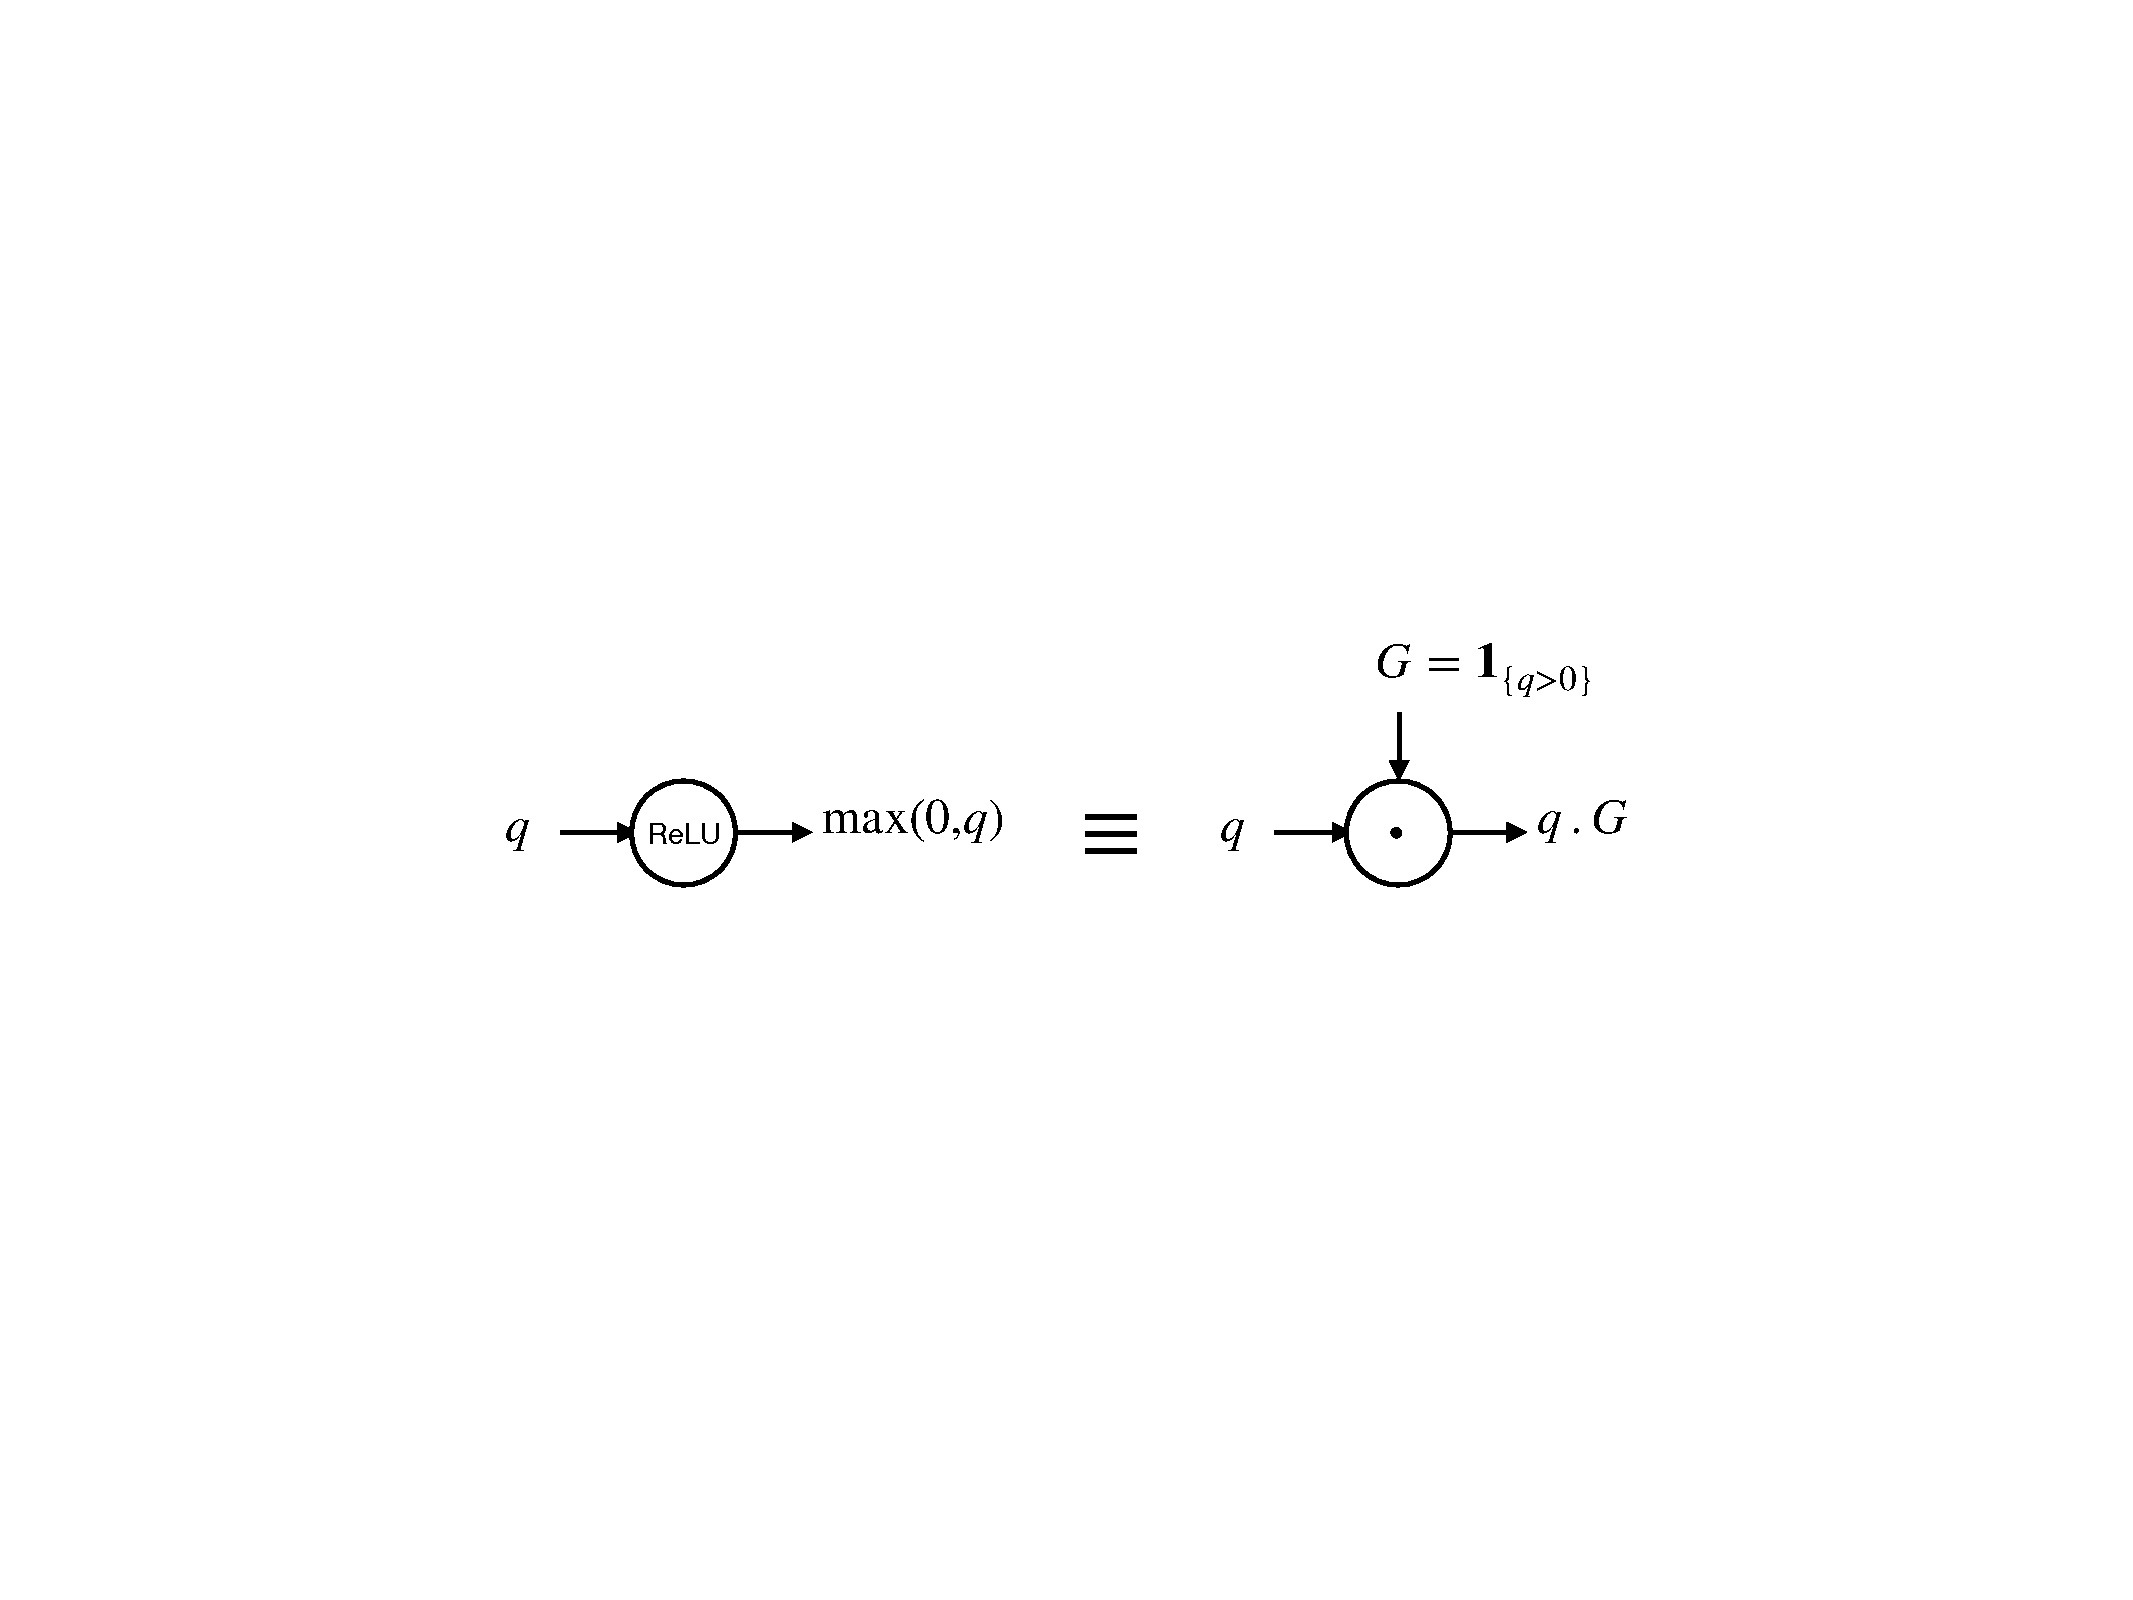
\includegraphics[scale=0.25]{figs/gating.pdf}
\caption{Gating property of ReLU}
\label{fig:gating}
\end{figure}
\subsection{Primal View: Layer by Layer}\label{sec:primal}
The layer-by-layer way of expressing the computation in a DNN of width `$w$' and depth `$d$' is given below.
\begin{table}[h]
\centering
\begin{tabular}{| lll|}\hline
 $z_{x,\Theta}(\cdot,0)$ &$=$ &$x$ \\
 $q_{x,\Theta}(\iout,l)$& $=$ & $\sum_{\iin}\Theta(\iin,\iout,l) \cdot z_{x,\Theta}(\iin,l-1) $\\
$G_{x,\Theta}(\iout,l)$& $=$ & $\mathbf{1}_{\{q_{x,\Theta}(\iout,l)>0\}}$\\
 $z_{x,\Theta}(\iout,l)$ & $=$ & $q_{x,\Theta}(\iout,l)\cdot G_{x,\Theta}(\iout,l)$\\
 $\hat{y}_{\Theta}(x)$ & $=$ & $\sum_{\iin}\Theta(\iin,\iout, d)\cdot z_{x,\Theta}(\iin,d-1)$\\\hline
\end{tabular}
\caption{\small{Information flow in a FC-DNN with ReLU. Here, `$q$'s are pre-activation inputs, `$z$'s are output of the hidden layers, `$G$'s are the gating values. $l\in[d-1]$ is the index of the layer, $\iout$ and $\iin$ are indices of  nodes in the current and previous layer respectively.}}
\label{tb:basic}
\end{table}

\subsection{Dual View: Path, Neural Path Feature and Value}\label{sec:dual}
\FloatBarrier
\begin{figure}[h]
\centering
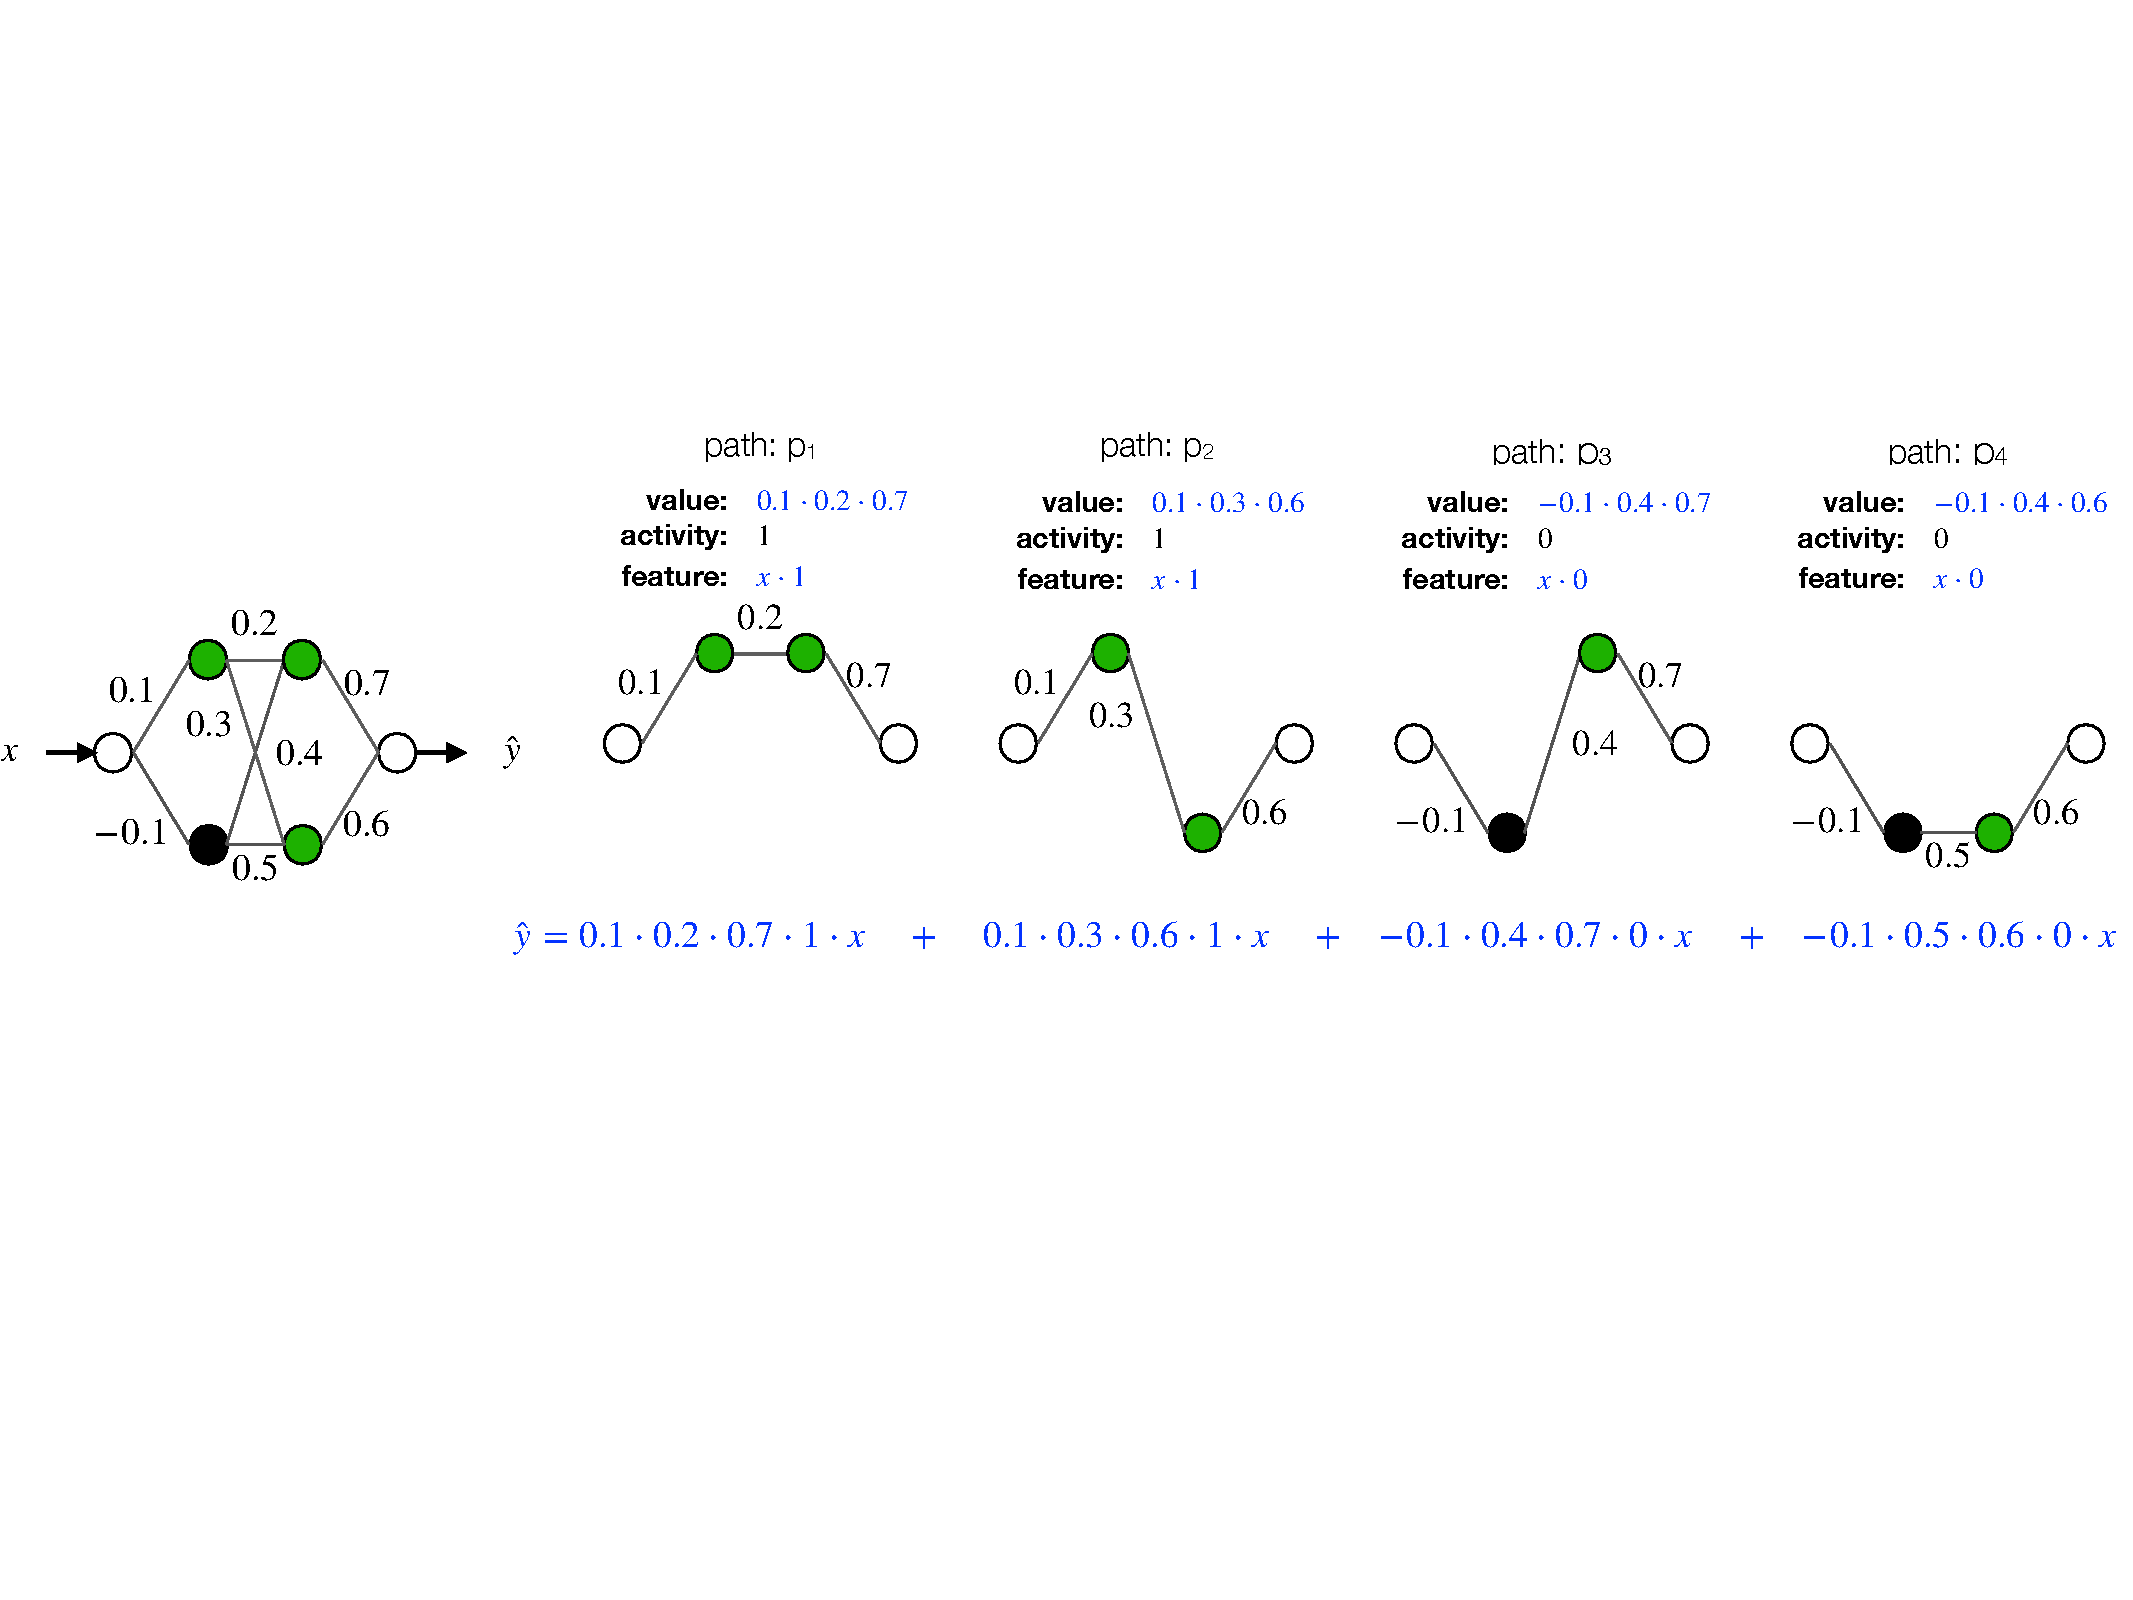
\includegraphics[scale=0.32]{figs/paths.pdf}
\caption{The thick line shows an arbitrary path.}
\end{figure}

\begin{definition}
A path starts from an input node, passes through a weight and a hidden node in each layer and ends at the output node.
\end{definition}
\begin{proposition}
FC-DNN has $\Pfc=\din w^{(d-1)}$ paths.
\end{proposition}
\begin{notation}
Index maps identify the nodes through which a path $p$ passes. The ranges of index maps $\Ifeat_l$, $\I_l,l\in[d-1]$ are $[\din]$ and $[w]$ respectively.  $\I_d(p)=1,\forall p\in[\Pfc]$.
\end{notation}

\begin{definition}\label{def:nps} Let $x\in\R^{\din}$ be the input to the DNN. For this input, 

(i)  $A_{\Theta}(x,p)\eqdef\Pi_{l=1}^{d-1} G_{x,\Theta}(\I_l(p),l)$ is the activity of a path.

(ii)  $\phi_{x,\Theta}\eqdef \left( x(\Ifeat_0(p))A_{\Theta}(x,p), p\in[\Pfc]\right)\in\R^{\Pfc}$ is the {neural path feature} (NPF).

(iii)  $v_{\Theta}\eqdef \left( \Pi_{l=1}^d \Theta(\I_{l-1}(p),\I_l(p),l), p\in[\Pfc]\right)\in\R^{\Pfc}$ is the {neural path value} (NPV).
\end{definition}
\textbf{Remark:} $\Ifeat_0(p)$ denotes the input node of path $p$. A coordinate of NPF can be non-zero only if the corresponding path is active ($A_{\Theta}(x,p)=1$), i.e., all the gates in the path are $1$. 
\begin{proposition}\label{prop:zero}  The output of the DNN can be written as an inner product of the NPF and NPV, i.e., 
$\hat{y}_{\Theta}(x)=\ip{\phi_{x,\Theta},v_{\Theta}}=\sum_{p\in [\Pfc]}x(\Ifeat_0(p))A_{\Theta}(x,p)v_{\Theta}(p)$.
\end{proposition}
The following result connects the NPFs and the NTK.
\begin{proposition}\label{prop:ntknew}
Let $\nabla_{\Theta}v_{\Theta}=(\varphi_{p,\Theta},p\in[\Pfc])$. Then NTK is given by $K_{\Theta}(x,x')=\phi^\top_{x,\Theta}(\nabla_{\Theta}v_{\Theta})^\top(\nabla_{\Theta}v_{\Theta})\phi_{x',\Theta}$.
\end{proposition}
\Cref{prop:ntknew} can be interpreted as the NTK being equal to the inner product of the NPFs with respect to a $\Pfc\times \Pfc$ positive semi-definite matrix $(\nabla_{\Theta}v_{\Theta})^\top(\nabla_{\Theta}v_{\Theta})$ which is solely dependent on the weights of the network.

